\documentclass{beamer}

\usepackage[utf8x]{inputenc}
\usepackage{graphicx}
\usepackage{amsthm,amssymb,amsbsy,amsmath,amsfonts,amssymb,amscd}
\usepackage{dsfont}
\usepackage{array}
\usepackage{verbatim}
\newcolumntype{N}{@{}m{2pt}@{}}
\usepackage{tikz}
%\usetikzlibrary{arrows}
%\tikzstyle{block}=[draw opacity=0.7,line width=1.4cm]

\input{style.tex} 

%\usepackage{xcolor}
\definecolor{Orange}{rgb}{0.8,0.1470,0.0}
\definecolor{MonBleu}{rgb}{0.212, 0.392, 0.545}


\title[ENBIS workshop: Introduction to Kriging 1/2]{ \small ENBIS pre-conference workshop\\ \vspace{3mm} \Large Introduction to Kriging using R and JMP }
\author[11th of Septembre 2016]{Nicolas Durrande -- Mines Saint-Étienne}
\institute{durrande@emse.fr}
\date{\null}

\DeclareMathOperator*{\Var}{var}
\DeclareMathOperator*{\E}{E}
\DeclareMathOperator*{\Cov}{cov}
\newcommand\PR[1]{\mathrm{P}\left(#1 \right)}
\newcommand\PS[1]{{\langle #1 \rangle}_\mathcal{H}}
\newcommand\PSi[2]{{ \left \langle #1 \right \rangle}_{\! #2}}
\newcommand\N[1]{{|| #1 ||}_\mathcal{H}}
\newcommand\Ni[2]{{|| #1 ||}_{\! #2}}
\newcommand\dx{\, \mathrm{d}}
\newcommand\textequal{\rule[.4ex]{4pt}{0.4pt}\llap{\rule[.7ex]{4pt}{0.4pt}}}
\newcommand{\argmin}{\operatornamewithlimits{argmin}}
\makeatletter
\newcommand{\shorteq}{%
  \settowidth{\@tempdima}{a}% Width of hyphen
  \resizebox{\@tempdima}{\height}{=}%
}
\makeatother

%%%%%%%%%%%%%%%%%%%%%%%%%%%%%%%%%%%%%%%%%%%%%%%%%%%%%%
%%%%%%%%%%%%%%%%%%%%%%%%%%%%%%%%%%%%%%%%%%%%%%%%%%%%%%
%%%%%%%%%%%%%%%%%%%%%%%%%%%%%%%%%%%%%%%%%%%%%%%%%%%%%%
\begin{document}
\setbeamercolor{author in head/foot}{fg=gray,bg=white}
\setbeamercolor{title in head/foot}{fg=gray,bg=white}
\setbeamercolor{page number in head/foot}{fg=gray,bg=white}
\setbeamercolor{section in head/foot}{bg=black,fg=gray}
\setbeamercolor{subsection in head/foot}{bg=black,fg=gray}

%%%%%%%%%%%%%%%%%%%%%%%%%%%%%%%%%%%%%%%%%%%%%%%%%%%%%%
\begin{frame}
  \titlepage
\end{frame}

%%%%%%%%%%%%%%%%%%%%%%%%%%%%%%%%%%%%%%%%%%%%%%%%%%%%%%
%%%%%%%%%%%%%%%%%%%%%%%%%%%%%%%%%%%%%%%%%%%%%%%%%%%%%%
\section[Context]{Context}
%\subsection{}

%%%%%%%%%%%%%%%%%%%%%%%%%%%%%%%%%%%%%%%%%%%%%%%%%%%%%%
\begin{frame}{}
There is a wide variety of situations where getting data is extremely expensive.
\begin{columns}[c]
\column{5cm}
\begin{itemize}
	\item real world experiments
	\item destructive tests
\end{itemize}
\column{5cm}
\begin{itemize}
	\item prototyping
	\item numerical experiments
\end{itemize}
\end{columns}

\begin{center}
\includegraphics[height=3.5cm]{figures/crash-test} \qquad \includegraphics[height=3.5cm]{figures/image15}
\end{center}
The number of experiments is thus limited.
\end{frame}

%%%%%%%%%%%%%%%%%%%%%%%%%%%%%%%%%%%%%%%%%%%%%%%%%%%%%%
\begin{frame}{}
During the lab session, we will consider a numerical simulator of a catapult depending on 4 inputs $ x_1,\dots,x_4 \in [0,1]$.
\begin{center}
\includegraphics[width=\textwidth]{figures/catapult_settings}
\end{center}
\end{frame}

%%%%%%%%%%%%%%%%%%%%%%%%%%%%%%%%%%%%%%%%%%%%%%%%%%%%%%
\begin{frame}{}
This numerical simulator returns the length and height of the throw
\begin{center}
\includegraphics[width=\textwidth]{figures/catapult_trajectory}
\end{center}
\end{frame}

%%%%%%%%%%%%%%%%%%%%%%%%%%%%%%%%%%%%%%%%%%%%%%%%%%%%%%
\begin{frame}{}
\begin{exampleblock}{Lab session R (5 min)}
	\begin{enumerate}
		\item Download and open the file ``morning\_lab.R'' from Nicolas Durrande's homepage
		\begin{center}
			{\scriptsize \url{https://sites.google.com/site/nicolasdurrandehomepage/shortcourses}}
		\end{center} 
		
		\item Execute the first two uncommented lines. %You may need to install the \texttt{shiny} package: \texttt{install.packages("shiny")}.
	\end{enumerate}
\end{exampleblock}
\bigskip
\begin{exampleblock}{Lab session JMP (5 min)}
	\begin{enumerate}
		\item do as above... 
	\end{enumerate}
	\begin{itemize}
		\item[or]
	\end{itemize}
	\begin{enumerate}
		\item go to: \url{https://durrande.shinyapps.io/catapult} 
	\end{enumerate}
\end{exampleblock}

\end{frame}

%%%%%%%%%%%%%%%%%%%%%%%%%%%%%%%%%%%%%%%%%%%%%%%%%%%%%%
\begin{frame}{}
The experiment output can be seen as a function of the input parameters
$$ y = f(x). $$
where $f$ is a \textbf{costly to evaluate function}. \\
\vspace{5mm}
In the following, we will assume that 
\begin{itemize}
	\item $x \in \mathds{R}^d$: There are many input parameters
	\item $y \in \mathds{R}$: The output is a scalar.
\end{itemize}
\end{frame}

%%%%%%%%%%%%%%%%%%%%%%%%%%%%%%%%%%%%%%%%%%%%%%%%%%%%%%
\begin{frame}{}
The fact that $f$ is \textbf{costly to evaluate} changes a lot of things...\\
\vspace{5mm}
\structure{1. Ploting the function is not possible...}\\
\vspace{5mm}
\begin{center}
\includegraphics[height=3.2cm]{figures/ink_f} \includegraphics[height=3.2cm]{figures/Rightarrow} \includegraphics[height=3.2cm]{figures/ink_fX}
\end{center}
\end{frame}

%%%%%%%%%%%%%%%%%%%%%%%%%%%%%%%%%%%%%%%%%%%%%%%%%%%%%%
\begin{frame}{}
The fact that $f$ is \textbf{costly to evaluate} changes a lot of things...\\
\vspace{5mm}
\structure{2. Computing integrals is not possible...}\\
\vspace{5mm}
\begin{center}
\includegraphics[height=4.5cm]{figures/ink_fX}
\end{center}
What is the mean value of $f$?
\end{frame}

%%%%%%%%%%%%%%%%%%%%%%%%%%%%%%%%%%%%%%%%%%%%%%%%%%%%%%
\begin{frame}{}
The fact that $f$ is \textbf{costly to evaluate} changes a lot of things...\\
\vspace{5mm}
\structure{3. Uncertainty propagation is not possible...}\\
\vspace{5mm}
\begin{center}
\includegraphics[height=3.2cm]{figures/ink_unprogf} \includegraphics[height=3.2cm]{figures/Rightarrow} \includegraphics[height=3.2cm]{figures/ink_unprogfX}
\end{center}
\end{frame}

%%%%%%%%%%%%%%%%%%%%%%%%%%%%%%%%%%%%%%%%%%%%%%%%%%%%%%
\begin{frame}{}
The fact that $f$ is \textbf{costly to evaluate} changes a lot of things...\\
\vspace{5mm}
\structure{4. Sensitivity analysis is not possible...}\\
\vspace{5mm}
\begin{center}
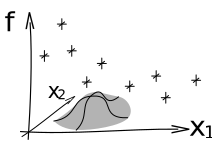
\includegraphics[height=4.5cm]{figures/ink_as2}
\end{center}
\end{frame}

%%%%%%%%%%%%%%%%%%%%%%%%%%%%%%%%%%%%%%%%%%%%%%%%%%%%%%
\begin{frame}{}
The fact that $f$ is \textbf{costly to evaluate} changes a lot of things...\\
\vspace{5mm}
\structure{5. Optimisation is also tricky...}\\
\vspace{5mm}
\begin{center}
\includegraphics[height=4.5cm]{figures/ink_fX}
\end{center}
\end{frame}

%%%%%%%%%%%%%%%%%%%%%%%%%%%%%%%%%%%%%%%%%%%%%%%%%%%%%%
%%%%%%%%%%%%%%%%%%%%%%%%%%%%%%%%%%%%%%%%%%%%%%%%%%%%%%
\section[Surrogates]{Surrogate models}
%\subsection{}

%%%%%%%%%%%%%%%%%%%%%%%%%%%%%%%%%%%%%%%%%%%%%%%%%%%%%%
\begin{frame}{}
The principle of statistical modelling is to use a few observations to build a mathematical approximation of the function. 
\begin{center}
\includegraphics[height=4.5cm]{figures/ink_m}
\end{center}
The model can then be used to answer all previous questions
\end{frame}

%%%%%%%%%%%%%%%%%%%%%%%%%%%%%%%%%%%%%%%%%%%%%%%%%%%%%%
\begin{frame}{}
Of course, there is a difference between $f$ and $m$...
\begin{center}
\includegraphics[height=5cm]{figures/ink_mf}
\end{center}
\end{frame}

%%%%%%%%%%%%%%%%%%%%%%%%%%%%%%%%%%%%%%%%%%%%%%%%%%%%%%
\begin{frame}{}
What about \textbf{statistical models}? \\We want to be able to quantify the model error:
\begin{center}
\includegraphics[height=5cm]{figures/ink_mconfint}
\end{center}
The confidence intervals can be used to obtain a \textbf{measure of uncertainty on the value of interest}.
\end{frame}

%%%%%%%%%%%%%%%%%%%%%%%%%%%%%%%%%%%%%%%%%%%%%%%%%%%%%%
\begin{frame}{}
There are many kinds of surrogate models:
\begin{columns}[t]
\column{4cm}
\begin{itemize}
	\item linear regression
	\item polynomial chaos
	% \item wavelets
\end{itemize}
\column{6cm}
\begin{itemize}
	\item neural networks
	\item Kriging (or Gaussian process regression)
\end{itemize}
\end{columns}
\begin{center}
\includegraphics[height=4.5cm]{figures/ink_m}
\end{center}
% We will use the following notations : 
% \begin{itemize}
% 	\item The set of observation points will be represented by a $n \times d$ matrix $X=(X_1, ..., X_n)^t$
% 	\item The vector of observations will be denoted by $F$ : $F_i=f(X_i)$ (or $F=f(X)$).
% \end{itemize}
\end{frame}

%%%%%%%%%%%%%%%%%%%%%%%%%%%%%%%%%%%%%%%%%%%%%%%%%%%%%%
\begin{frame}{}
\begin{exampleblock}{Example: linear regression for the catapult simulator}
We consider the simulator as a function of only $x_1$ and $x_2$ and 16 observation points where the simulator will be run: 
\begin{columns}[c]
\column{3cm}
\begin{equation*}
	X = 
	\begin{pmatrix}
		0.00 & 0.00 \\
		0.33 & 0.00 \\
		0.66 & 0.00 \\
		1.00 & 0.00 \\
		0.00 & 0.33 \\
		\vdots&\vdots\\
		1.00 & 1.00\\
	\end{pmatrix}
\end{equation*}
\column{5cm}
\begin{center}
\includegraphics[height=5cm]{figures/R/linReg_DoE}
\end{center}
\end{columns}
\end{exampleblock}
\end{frame}

%%%%%%%%%%%%%%%%%%%%%%%%%%%%%%%%%%%%%%%%%%%%%%%%%%%%%%
\begin{frame}{}
\begin{exampleblock}{Example: linear regression for the catapult simulator}
We run the simulator (variables $x_3$ and $x_4$ are set to 0.5). We obtain
\begin{columns}[c]
\column{1cm}
\begin{equation*}
	Y =
	\begin{pmatrix}
		 57.8 \\
		 30.1 \\
		 12.4 \\
		  1.2 \\
		126.2 \\
		\vdots\\
		111.0\\
	\end{pmatrix} 
\end{equation*}
\column{5cm}
\begin{center}
\includegraphics[height=6cm]{figures/R/linReg_output.png}
\end{center}
\end{columns}
\end{exampleblock}
\end{frame}

%%%%%%%%%%%%%%%%%%%%%%%%%%%%%%%%%%%%%%%%%%%%%%%%%%%%%%
\begin{frame}[fragile]{}
\begin{exampleblock}{Example: linear regression for the catapult simulator}
We assume the following linear regression model
$$Y_i = \beta_0 + \beta_1 X_{i,1} + \beta_2 X_{i,2} + \varepsilon_i$$
where the $\beta_k$ are unknown and the $\varepsilon_i$ are $\mathcal{N}(0,\sigma^2)$ and independents.\\
\vspace{5mm}
The $\beta_k$ can be estimated by minimising the residual sum of squares:
\begin{verbatim}
	> XY <- data.frame(x1=X[,1],x2=X[,2],y=Y)
	> mr <- lm(y ~ 1 + x1 + x2, data = XY)   
\end{verbatim}
\end{exampleblock}
\end{frame}


%%%%%%%%%%%%%%%%%%%%%%%%%%%%%%%%%%%%%%%%%%%%%%%%%%%%%%
\begin{frame}[fragile]{}
\begin{exampleblock}{Example: linear regression for the catapult simulator}
We obtain $\beta = (62.76,\ -59.71,\ 95.30 )$ :
\begin{verbatim}
	> summary(mr)
\end{verbatim}
{\footnotesize
\begin{verbatim}
Residuals:
    Min      1Q  Median      3Q     Max 
-78.011 -11.058  -3.427  15.187  35.165 

Coefficients:
            Estimate Std. Error t value Pr(>|t|)    
(Intercept)    62.76      15.66   4.008  0.00149 ** 
x1            -59.71      19.67  -3.035  0.00957 ** 
x2             95.30      19.67   4.845  0.00032 ***
---
Signif. codes:  0 ‘***’ 0.001 ‘**’ 0.01 ‘*’ 0.05 ‘.’ 0.1 ‘ ’ 1

Residual standard error: 29.3 on 13 degrees of freedom
Multiple R-squared:  0.7155,	Adjusted R-squared:  0.6717 
F-statistic: 16.34 on 2 and 13 DF,  p-value: 0.0002832
\end{verbatim}
}
\end{exampleblock}
\end{frame}

%%%%%%%%%%%%%%%%%%%%%%%%%%%%%%%%%%%%%%%%%%%%%%%%%%%%%%
\begin{frame}{}
\begin{exampleblock}{Example: linear regression for the catapult simulator}
\begin{center}
\includegraphics[height=6cm]{figures/R/linReg_model.png}
\end{center}
\end{exampleblock}
\end{frame}

%%%%%%%%%%%%%%%%%%%%%%%%%%%%%%%%%%%%%%%%%%%%%%%%%%%%%%
\begin{frame}[fragile]{}
\begin{exampleblock}{Example: linear regression for the catapult simulator}
The model can be improved by changing the basis functions:
 $$\phi_0 = 1,\ \phi_1 = x_1-x_2,\ \phi_2 = (x_1-x_2)^2,\text{ and } \phi_3 = (x_1-x_2)^3.$$
{\footnotesize
\begin{verbatim}
Residuals:
    Min      1Q  Median      3Q     Max 
-35.042  -8.153   2.001   9.579  20.957 

Coefficients:
               Estimate Std. Error t value Pr(>|t|)    
(Intercept)      92.836      5.386  17.236 7.86e-10 ***
I(x1 - x2)     -147.913     16.510  -8.959 1.16e-06 ***
I((x1 - x2)^2)  -44.608     12.747  -3.500 0.004386 ** 
I((x1 - x2)^3)  109.325     22.661   4.824 0.000416 ***
---
Signif. codes:  0 ‘***’ 0.001 ‘**’ 0.01 ‘*’ 0.05 ‘.’ 0.1 ‘ ’ 1

Residual standard error: 16.26 on 12 degrees of freedom
Multiple R-squared:  0.9191,	Adjusted R-squared:  0.8989 
F-statistic: 45.44 on 3 and 12 DF,  p-value: 7.933e-07
\end{verbatim}
}
\end{exampleblock}
\end{frame}

%%%%%%%%%%%%%%%%%%%%%%%%%%%%%%%%%%%%%%%%%%%%%%%%%%%%%%
\begin{frame}{}
\begin{exampleblock}{Example: linear regression for the catapult simulator}
\begin{center}
\includegraphics[height=6cm]{figures/R/linReg_model2.png}
\end{center}
\end{exampleblock}
\end{frame}

% %%%%%%%%%%%%%%%%%%%%%%%%%%%%%%%%%%%%%%%%%%%%%%%%%%%%%%
% \begin{frame}[fragile]{}
% \begin{exampleblock}{Example: linear regression for the catapult simulator}
% We consider 16 observation points located at the $[0,1]^4$ corners. 
% \begin{equation*}
% 	X = 
% 	\begin{pmatrix}
% 		0&0&0&0\\
% 		1&0&0&0\\
% 		0&1&0&0\\
% 		1&1&0&0\\
% 		0&0&1&0\\
% 		\vdots&\vdots&\vdots&\vdots\\
% 		1&1&1&1\\
% 	\end{pmatrix}
% 	\qquad \qquad Y =
% 		\begin{pmatrix}
% 		54.7 \\
% 		 0.6 \\
% 		73.9 \\
% 		95.7 \\
% 		50.7 \\
% 		\vdots\\
% 		121.3\\
% 	\end{pmatrix} 
% \end{equation*}
% \end{exampleblock}
% \end{frame}

% %%%%%%%%%%%%%%%%%%%%%%%%%%%%%%%%%%%%%%%%%%%%%%%%%%%%%%
% \begin{frame}[fragile]{}
% \begin{exampleblock}{Example: linear regression for the catapult simulator}
% We assume the following linear regression model
% $$Y_i = \beta_0 + \sum_{k=1}^d \beta_k X_{i,k} + \varepsilon_i$$
% where the $\beta_k$ are unknown and the $\varepsilon_i$ are $\mathcal{N}(0,\sigma^2)$ and independents.\\
% \vspace{5mm}
% The $\beta_k$ can be estimated by minimising the residual sum of squares:
% {\small
% \begin{verbatim}
% 	XY <- data.frame(x1=X[,1],x2=X[,2],x3=X[,3],x4 = X[,4],y=Y)
% 	mr <- lm(y ~ ., data = XY)   
% 	summary(mr)
% \end{verbatim}
% }
% \end{exampleblock}
% \end{frame}

% %%%%%%%%%%%%%%%%%%%%%%%%%%%%%%%%%%%%%%%%%%%%%%%%%%%%%%
% \begin{frame}[fragile]{}
% \begin{exampleblock}{Example: linear regression for the catapult simulator}
% We obtain $\beta = (30.6,\ -13.2,\ 65.8,\ -2.7,\ 13.0)$ :
% {\footnotesize
% \begin{verbatim}
% Residuals:
%     Min      1Q  Median      3Q     Max 
% -27.141 -20.821  -1.343  22.237  32.391 

% Coefficients:
%             Estimate Std. Error t value Pr(>|t|)    
% (Intercept)   30.550     14.953   2.043 0.065748 .  
% x1           -13.191     13.374  -0.986 0.345166    
% x2            65.759     13.374   4.917 0.000459 ***
% x3            -2.703     13.374  -0.202 0.843523    
% x4            13.025     13.374   0.974 0.351025    
% ---
% Signif. codes:  0 ‘***’ 0.001 ‘**’ 0.01 ‘*’ 0.05 ‘.’ 0.1 ‘ ’ 1

% Residual standard error: 26.75 on 11 degrees of freedom
% Multiple R-squared:  0.7038,	Adjusted R-squared:  0.5961 
% F-statistic: 6.535 on 4 and 11 DF,  p-value: 0.006043
% \end{verbatim}
% }
% \end{exampleblock}
% \end{frame}

% %%%%%%%%%%%%%%%%%%%%%%%%%%%%%%%%%%%%%%%%%%%%%%%%%%%%%%
% \begin{frame}[fragile]{}
% \begin{exampleblock}{Example: linear regression for the catapult simulator}
% Let's assume another linear regression model
% $$Y_i = \beta_0 + \beta_1 X_{i,1} + \beta_2 X_{i,2} + \beta_3 X_{i,1} \times X_{i,2} + \varepsilon_i$$
% {\footnotesize
% \begin{verbatim}
% Residuals:
%      Min       1Q   Median       3Q      Max 
% -16.2813  -5.0420  -0.2658   4.9065  18.7709 

% Coefficients:
%             Estimate Std. Error t value Pr(>|t|)    
% (Intercept)   57.195      4.986  11.472 7.97e-08 ***
% x1           -56.159      7.051  -7.965 3.93e-06 ***
% x2            22.791      7.051   3.232  0.00719 ** 
% x1:x2         85.935      9.971   8.618 1.74e-06 ***
% ---
% Signif. codes:  0 ‘***’ 0.001 ‘**’ 0.01 ‘*’ 0.05 ‘.’ 0.1 ‘ ’ 1

% Residual standard error: 9.971 on 12 degrees of freedom
% Multiple R-squared:  0.9551,	Adjusted R-squared:  0.9439 
% F-statistic: 85.08 on 3 and 12 DF,  p-value: 2.357e-08
% \end{verbatim}
% }
% \end{exampleblock}
% \end{frame}

%%%%%%%%%%%%%%%%%%%%%%%%%%%%%%%%%%%%%%%%%%%%%%%%%%%%%%
\begin{frame}{}
One can distinguish 4 important steps for building a surrogate model :
\begin{enumerate}
	\item Choosing the evaluation points (Design of Experiments)
	\item Evaluating the costly function
	\item Choosing the type of model and estimating its parameters 
	\item Validating the model
	\item Computing the quantity of interest
\end{enumerate}
We will now detail these, with a focus on Kriging models.
\end{frame}

%%%%%%%%%%%%%%%%%%%%%%%%%%%%%%%%%%%%%%%%%%%%%%%%%%%%%%
%%%%%%%%%%%%%%%%%%%%%%%%%%%%%%%%%%%%%%%%%%%%%%%%%%%%%%
\section[DoE]{Design of experiments}
%\subsection{}

%%%%%%%%%%%%%%%%%%%%%%%%%%%%%%%%%%%%%%%%%%%%%%%%%%%%%%
\frame{
  \frametitle{Design specificities for computer experiments}
  Two main constraints and their consequences.
  \bigskip
  \begin{enumerate}
  \item For deterministic simulators, running twice the simulator at
    the same location gives the same result 
    \begin{itemize}
    	\item[$\rightarrow$] \structure{Avoid replications}
    \end{itemize}
  \item A simulator generally models a complex phenomenon with
    strongly non-linear behaviour
        \begin{itemize}
    	\item[$\rightarrow$] \structure{Fill the space, in order to avoid missing an area}
    \end{itemize}
  \end{enumerate}
}

%%%%%%%%%%%%%%%%%%%%%%%%%%%%%%%%%%%%%%%%%%%%%%%%%%%%%%
\frame{
  \frametitle{}
  Additional constraint: 
  \begin{enumerate}
    \setcounter{enumi}{2}
  \item The aforementioned principles should apply in lower subspaces,
    since the \emph{true} dimensionality can be lower.
  \end{enumerate}
  \bigskip
  
  Example: $f_{\text{sim}}(x_1, x_2) = g(x_1)$
  \begin{itemize}
  	\item[$\rightarrow$] \structure{It is useless to run the simulator with same $x_1$ locations!}
  	\item[$\rightarrow$] \structure{The $x_1$ locations should fill the space}
  \end{itemize}
}

%%%%%%%%%%%%%%%%%%%%%%%%%%%%%%%%%%%%%%%%%%%%%%%%%%%%%%
\frame{
  \frametitle{A potentially bad design: How to waste 2/3 of runs!}
  \bigskip
  Only 3 points among 9 are useful if $f_{\text{sim}}$ depends only on $x_1$ (or $x_2$).
  \includegraphics[width=6cm]{figures/R/DoE_grid}
  \includegraphics[width=6cm]{figures/R/DoE_gridarrow}
}

%%%%%%%%%%%%%%%%%%%%%%%%%%%%%%%%%%%%%%%%%%%%%%%%%%%%%%
\begin{frame}{}
Various design types can be found in the literature:
\begin{itemize}
	\item Latin Hypercubes
	\item Low discrepancy sequences
	\item Voronoi Tessellations
	\item ...
\end{itemize}
Various criteria can be used to asses a DoE quality
\begin{itemize}
	\item Maximin
	\item Minimax
	\item Discrepancy
	\item IMSE
	\item ...
\end{itemize}
Some of them are implemented in the \texttt{DiceDesign package}
\end{frame}

%%%%%%%%%%%%%%%%%%%%%%%%%%%%%%%%%%%%%%%%%%%%%%%%%%%%%%
\begin{frame}[fragile]{Better designs: Latin hypercubes}
  \begin{verbatim}
  	library(DiceDesign)
  	X <- lhsDesign(n = 9, dimension = 2, seed = 3,
  	                 randomized = FALSE)$design
  \end{verbatim}
  %\vspace{-15mm}
  \begin{center}
  \includegraphics[width=5cm]<1>{figures/R/DoE_LHS}
  \includegraphics[width=5cm]<2>{figures/R/DoE_LHSarrow}
  \end{center}
\end{frame}

%%%%%%%%%%%%%%%%%%%%%%%%%%%%%%%%%%%%%%%%%%%%%%%%%%%%%%
\begin{frame}[fragile]{Good(?) designs: space-filling Latin hypercubes}
  \begin{verbatim}
  X0 <- lhsDesign(n = 9, dimension = 2)$design
  X <- maximinESE_LHS(X0, it=2)$design
  \end{verbatim}
  \begin{center}
  \includegraphics[width=5cm]{figures/R/DoE_LHSmaximin}
  \end{center}
\end{frame}

%%%%%%%%%%%%%%%%%%%%%%%%%%%%%%%%%%%%%%%%%%%%%%%%%%%%%%
\begin{frame}{}
\small
\begin{columns}[t]
\column{5cm}
\begin{exampleblock}{Lab session R (25 min)}
	\begin{enumerate}
		\item Load the DiceDesign package and build a DoE of 16 points in $[0,1]^4$. Store it in a $16 \times 4$ matrix \texttt{X}.
		\item Plot the columns of \texttt{X} against each other (\texttt{pairs(X)}).
		\item Use the numerical simulator to compute the output values. Store them in a vector \texttt{Y}.
		\item plot \texttt{Y} against the various input variables.
		\item What optimal input values can you suggest?
		$$ x_1 = \qquad,\ x_2 = \qquad,\ x_3 = \qquad,\ x_4 = \qquad.$$
	\end{enumerate}
\end{exampleblock}
\column{5cm}
\begin{exampleblock}{Lab session JMP (25 min)}
	\begin{enumerate}
		\item Open the file \emph{Intro\_to\_Kriging\_JMP.jrn}
		\item Repeat the previous trials with a linear regression model.
		\item Create a Design of experiments.
		\item Use the numerical simulator to compute the output values. Store them in a vector \texttt{Y}.
		\item plot \texttt{Y} against the various input variables.
		\item What optimal input values can you suggest?
		$$ x_1 = \qquad,\ x_2 = \qquad,\ x_3 = \qquad,\ x_4 = \qquad.$$
	\end{enumerate}
\end{exampleblock}
\end{columns}

\end{frame}

%%%%%%%%%%%%%%%%%%%%%%%%%%%%%%%%%%%%%%%%%%%%%%%%%%%%%%
%%%%%%%%%%%%%%%%%%%%%%%%%%%%%%%%%%%%%%%%%%%%%%%%%%%%%%
\section[Kriging]{Kriging or Gaussian process regression}
%\subsection{}

%%%%%%%%%%%%%%%%%%%%%%%%%%%%%%%%%%%%%%%%%%%%%%%%%%%%%%
\begin{frame}{}
A random process is similar to a random variable but each draw is a function:
\begin{center}
\includegraphics[height=6cm]{figures/R/GPR_GaussPrior}
\end{center}
Gaussian processes are particular random processes: $Z$ is a GP if any linear combination of $Z(x_i)$ is normally distributed.
\end{frame}

%%%%%%%%%%%%%%%%%%%%%%%%%%%%%%%%%%%%%%%%%%%%%%%%%%%%%%
\begin{frame}{}
The distribution of a
\begin{itemize}
	\item \textbf{Gaussian random variable} is fully described by its \emph{mean (scalar)} and \emph{variance (positive scalar)}.
	\item \textbf{Gaussian vector} (i.e. multivariate normal) is fully described by its \emph{mean vector} and \emph{covariance matrix} (symmetric positive semi-definite matrix).
	\item \textbf{Gaussian process} is fully described by its \emph{mean function} and \emph{covariance function} (or kernel):
	$$ k(x,y) = \Cov[Z(x),Z(y)] $$
\end{itemize}
\end{frame}

%%%%%%%%%%%%%%%%%%%%%%%%%%%%%%%%%%%%%%%%%%%%%%%%%%%%%%
\begin{frame}{}
The mean of a GP can be any function, but the kernel must satisfy two properties:
\begin{itemize}
	\item It is symmetric: $k(x,y) = k(y,x)$
	\item It is positive semi-definite (psd):
\end{itemize}
\begin{equation*}
	\forall n \in \mathds{N}, \forall x_i \in D, \forall \alpha \in \mathds{R}^n,\  \sum_{i=1}^n \sum_{j=1}^n \alpha_i \alpha_j k(x_i,x_j) \geq 0
\end{equation*}
This can be written in a matrix fashion:
\begin{equation*}
	\forall n \in \mathds{N}, \forall X \in D^n, \forall \alpha \in \mathds{R}^n,\  \alpha^t k(X,X) \alpha \geq 0
\end{equation*}
% \vspace{5mm}
Furthermore any symmetric psd function can be seen as the covariance of a Gaussian process. This equivalence is known as the Loeve theorem.
\end{frame}

%%%%%%%%%%%%%%%%%%%%%%%%%%%%%%%%%%%%%%%%%%%%%%%%%%%%%%
\begin{frame}{}
\begin{exampleblock}{Exercise}
Prove that the following functions are valid covariance functions
\begin{enumerate}
	\item $k(x,y) = 1$
	\item $k(x,y) = \delta_{x=y}$
	\item $k(x,y) = \exp(-(x-y)^2)$
\end{enumerate}	
\end{exampleblock}
\end{frame}

%%%%%%%%%%%%%%%%%%%%%%%%%%%%%%%%%%%%%%%%%%%%%%%%%%%%%%
\begin{frame}{}
\begin{exampleblock}{Exercise solutions}
\begin{columns}[c]
\column{7cm}
\begin{enumerate}
	\item It can be proved directly from the definition. This is the covariance of the following GP: \vspace{5mm}
	\item As above, it can be proved using the definition. This is the covariance function of the white noise process.\vspace{5mm}
	\item This cannot be proved from the definition, as for most kernels. However, this is a valid covariance function. 
\end{enumerate}	
\column{4cm}
\includegraphics[height=3.5cm]{figures/R/GPR_simCst}%Cst
\\
\vspace{7mm}
\includegraphics[height=3.5cm]{figures/R/GPR_simGauss}
\end{columns}
\end{exampleblock}
\end{frame}


%%%%%%%%%%%%%%%%%%%%%%%%%%%%%%%%%%%%%%%%%%%%%%%%%%%%%%
\begin{frame}{}
\vspace{5mm}
In order to plot sample paths from a GP $Z \sim \mathcal{N}(m(.),k(.,.))$, we will consider samples of the GP discretised on a fine grid.
\vspace{5mm}
\begin{exampleblock}{Exercise: Simulating sample paths}
Let X be a set 100 regularly spaced points over the input space of $Z$.
\begin{itemize}
	\item What is the distribution of $Z(X)$ ?
	\item How to simulate samples from $Z(X)$ ?
\end{itemize}
\end{exampleblock}
\end{frame}

%%%%%%%%%%%%%%%%%%%%%%%%%%%%%%%%%%%%%%%%%%%%%%%%%%%%%%
\begin{frame}{}
We have observed the function $f$ for a set of points $X = (X_1,\dots,X_n)$:
\begin{center}
\includegraphics[height=6cm]{figures/R/GPR_obs}
\end{center}
The vector of observations is $F=f(X)$ (ie $F_i = f(X_i)$ ).
\end{frame}

%%%%%%%%%%%%%%%%%%%%%%%%%%%%%%%%%%%%%%%%%%%%%%%%%%%%%%
\begin{frame}{}
We assume $f$ is a sample from a given GP and we know it interpolates... 
\begin{center}
\includegraphics[height=6cm]{figures/R/GPR_GaussBoth}
\end{center}
What can we say if we combine these two informations?
\end{frame}

%%%%%%%%%%%%%%%%%%%%%%%%%%%%%%%%%%%%%%%%%%%%%%%%%%%%%%
\begin{frame}{}
We obtain the following \textbf{conditional samples}:
\begin{center}
\includegraphics[height=6cm]{figures/R/GPR_GaussPosterior}
\end{center}
\end{frame}

%%%%%%%%%%%%%%%%%%%%%%%%%%%%%%%%%%%%%%%%%%%%%%%%%%%%%%
\begin{frame}{}
Which can be summarized by a mean function and confidence intervals:
\begin{center}
\includegraphics[height=6cm]{figures/R/GPR_GaussGPR}
\end{center}
\end{frame}

%%%%%%%%%%%%%%%%%%%%%%%%%%%%%%%%%%%%%%%%%%%%%%%%%%%%%%
\begin{frame}{}
The conditional distribution $Z(x)|Z(X) \shorteq F$ is still Gaussian and it can be computed analytically:\\
\vspace{2mm}
\textbf{mean value}
\begin{equation*}
	\begin{split}
		m(x) &= \E[Z(x)|Z(X) \shorteq F] \\
		&= k(x,X) k(X,X)^{-1} F
	\end{split}
\end{equation*}
\textbf{predicted variance}
\begin{equation*}
  \begin{split}
    v(x) &= \Var[Z(x)|Z(X) \shorteq F] \\
    &= k(x,x) - k(x,X) k(X,X)^{-1} k(X,x)
  \end{split}
\end{equation*}
\textbf{predicted covariance}
\begin{equation*}
  \begin{split}
    c(x,y) &= \Cov[Z(x),Z(y)|Z(X) \shorteq F] \\
    &= k(x,y) - k(x,X) k(X,X)^{-1} k(X,y)
  \end{split}
\end{equation*}
where $k(x,y) = \Cov[Z(x),Z(y)]$.
\end{frame}


%%%%%%%%%%%%%%%%%%%%%%%%%%%%%%%%%%%%%%%%%%%%%%%%%%%%%%
\begin{frame}{}
A few remarkable properties of GPR models 
\begin{itemize}
  \item They can interpolate the data-points
  \item The prediction variance does not depend on the observations
  \item The mean predictor does not depend on the variance
  \item The mean predictor (usually) comes back to zero when for predictions far away from the observations.
\end{itemize}
\end{frame}

%%%%%%%%%%%%%%%%%%%%%%%%%%%%%%%%%%%%%%%%%%%%%%%%%%%%%%
\begin{frame}{}
\begin{columns}[t]
\column{5cm}
\begin{exampleblock}{Lab session R (25 min)}
	\begin{enumerate}
		\item Load the \texttt{DiceKriging} package look at the help of the function \texttt{km}.
		\item Create a Kriging model on the catapult data with default kernel and parameters.
		\item Use the functions \texttt{sectionview} and \texttt{sectionview3d} from the package \texttt{DiceView}.
		\item Do some variables seem more influential than others?
	\end{enumerate}
\end{exampleblock}
\column{5cm}
\begin{exampleblock}{Lab session JMP (25 min)}
	\begin{enumerate}
		\item Create a Kriging model on the catapult data with default kernel and parameters.
		\item Explore the model using the diagnostics.
		\item Do some variables seem more influential than others?
	\end{enumerate}
\end{exampleblock}
\end{columns}
\end{frame}

%%%%%%%%%%%%%%%%%%%%%%%%%%%%%%%%%%%%%%%%%%%%%%%%%%%%%%
%%%%%%%%%%%%%%%%%%%%%%%%%%%%%%%%%%%%%%%%%%%%%%%%%%%%%%
\section{Model validation}
% \subsection{}

%%%%%%%%%%%%%%%%%%%%%%%%%%%%%%%%%%%%%%%%%%%%%%%%%%%%%%
\begin{frame}{}
We have seen that given some observations $F=f(X)$, it is very easy to build lots of models, either by changing the kernel parameters or the kernel itself.\\ \vspace{5mm}
The interesting question now is to know how to get a good model. To do so, we will need to answer the following questions:
\begin{itemize}
	\item What is a good model?
	\item How to measure it?
\end{itemize}
\end{frame}

%%%%%%%%%%%%%%%%%%%%%%%%%%%%%%%%%%%%%%%%%%%%%%%%%%%%%%
\begin{frame}{}
The idea is to introduce new data and to compare the model prediction with reality 
\begin{center}
\includegraphics[height=4.5cm]{figures/R/VALID_testset}
\end{center}
\vspace{3mm}
Since GPR models provide a mean and a covariance structure for the error they both have to be assessed.
\end{frame}

%%%%%%%%%%%%%%%%%%%%%%%%%%%%%%%%%%%%%%%%%%%%%%%%%%%%%%
\begin{frame}{}
Let $X_t$ be the test set and $F_t=f(X_t)$ be the associated observations.\\ \vspace{5mm}
The accuracy of the mean can be measured by computing: 
\begin{equation*}
	\begin{split}
		\text{Mean Square Error\qquad}& MSE = \mathrm{mean} ((F_t - m(X_t))^2) \\
		\text{A ``normalised'' criterion\qquad}& Q_2 = 1 - \frac{\sum (F_t - m(X_t))^2}{\sum (F_t - \mathrm{mean}(F_t))^2} 
	\end{split}
\end{equation*}
\\ \ \\
On the above example we get $MSE = 0.038$ and $Q_2 = 0.95$.
\end{frame}

%%%%%%%%%%%%%%%%%%%%%%%%%%%%%%%%%%%%%%%%%%%%%%%%%%%%%%
\begin{frame}{}
The predicted distribution can be tested by normalising the residuals. \\ \vspace{3mm}
According to the model, $F_t \sim \mathcal{N}(m(X_t),c(X_t,X_t))$.\\ \vspace{3mm}
$c(X_t,X_t)^{-1/2}(F_t-m(X_t)) $ should thus be independents $\mathcal{N}(0,1)$:
\begin{center}
\includegraphics[height=5cm]{figures/R/VALID_hist} \qquad
\includegraphics[height=5cm]{figures/R/VALID_qqplot}
\end{center}
\end{frame}

%%%%%%%%%%%%%%%%%%%%%%%%%%%%%%%%%%%%%%%%%%%%%%%%%%%%%%
\begin{frame}{}
When no test set is available, another option is to consider cross validation methods such as leave-one-out. \\ \vspace{5mm}
The steps are:
\begin{enumerate}
	\item[1.] build a model based on all observations except one
	\item[2.] compute the model error at this point
\end{enumerate}
This procedure can be repeated for all the design points in order to get a vector of error.\\ \vspace{3mm}
\end{frame}

%%%%%%%%%%%%%%%%%%%%%%%%%%%%%%%%%%%%%%%%%%%%%%%%%%%%%%
\begin{frame}{}
Model to be tested:\\ \vspace{3mm}
\begin{center}
\includegraphics[height=6cm]{figures/R/VALID_crossval0}
\end{center}
\end{frame}

%%%%%%%%%%%%%%%%%%%%%%%%%%%%%%%%%%%%%%%%%%%%%%%%%%%%%%
\begin{frame}{}
Step 1:\\ \vspace{3mm}
\begin{center}
\includegraphics[height=6cm]{figures/R/VALID_crossval1}
\end{center}
\end{frame}

%%%%%%%%%%%%%%%%%%%%%%%%%%%%%%%%%%%%%%%%%%%%%%%%%%%%%%
\begin{frame}{}
Step 2:\\ \vspace{3mm}
\begin{center}
\includegraphics[height=6cm]{figures/R/VALID_crossval2}
\end{center}
\end{frame}

%%%%%%%%%%%%%%%%%%%%%%%%%%%%%%%%%%%%%%%%%%%%%%%%%%%%%%
\begin{frame}{}
Step 3:\\ \vspace{3mm}
\begin{center}
\includegraphics[height=6cm]{figures/R/VALID_crossval3}
\end{center}
\end{frame}

%%%%%%%%%%%%%%%%%%%%%%%%%%%%%%%%%%%%%%%%%%%%%%%%%%%%%%
\begin{frame}{}
Leave one out often returns worst criteria values copared to test sets... \\
 \vspace{5mm}
We can also look at the residual distribution. For leave-one-out, there is no joint distribution for the residuals so they have to be standardised independently. We obtain: 
\begin{center}
\includegraphics[height=5cm]{figures/R/VALID_crossvalhist} \qquad
\includegraphics[height=5cm]{figures/R/VALID_crossvalqqplot}
\end{center}
\end{frame}



\end{document}













%%%%%%%%%%%%%%%%%%%%%%%%%%%%%%%%%%%%%%%%%%%%%%%%%%%%%%%%%%%%%%%%%%%%%%%%%%%%%%%
%%%%%%%%%%%%%%%%%%%%%%%%%%%%%%%%%%%%%%%%%%%%%%%%%%%%%%%%%%%%%%%%%%%%%%%%%%%%%%%
%%%%%%%%%%%%%%%%%%%%%%%%%%%%%%%%%%%%%%%%%%%%%%%%%%%%%%%%%%%%%%%%%%%%%%%%%%%%%%%
%%%%%%%%%%%%%%%%%%%%%%%%%%%%%%%%%%%%%%%%%%%%%%%%%%%%%%%%%%%%%%%%%%%%%%%%%%%%%%%
\end{document}



\structure{}

\begin{center}
  \begin{tabular}{|c|cc|}

  \end{tabular}
\end{center}

###
%%%%%%%%%%%%%%%%%%%%%%%%%%%%%%%%%%%%%%%%%%%%%%%%%%%%%%
\begin{frame}{}

\end{frame}

###
\begin{block}{}

\end{block}

###
\begin{center}
\includegraphics[height=5cm]{figures/}
\end{center}

###
\begin{columns}[c]
\column{5cm}

\column{5cm}

\end{columns}
